%% ============================================================
%%  Chapter (bridge) — Reproducibility, Degradation, and the
%%                     Device-Provenance Infrastructure
%%
%%  Author : Carlos David Prado-Socorro
%%  Date   : June 2026
%%  Institution : ICMol, Universitat de València
%%
%%  Compile with: latexmk -pdf  (standalone) or via thesis.tex
%%  Plan + evidence: handouts/22_bridge_chapter_plan.md,
%%                   scripts/bridge_hybrane_peo_reproducibility.py,
%%                   handouts/bridge_hybrane_peo_summary.csv
%% ============================================================

%% ---- Standalone preamble (skipped when \include'd from thesis.tex) ----
\ifdefined\thesismode\else
  \documentclass[12pt, twoside]{report}
  \usepackage{thesis-format}
  \addbibresource{../bibliography/references.bib}
  \begin{document}
  \setcounter{chapter}{2}     % This is Chapter 3 when built standalone
\fi

%% --- Shared macros (\providecommand: harmless if earlier chapters declared them) ---
\providecommand{\SY}{\textit{Super Yellow}}
\providecommand{\Hybrane}{\textit{Hybrane}}
\providecommand{\PEO}{PEO}
\providecommand{\LiTf}{LiOTf}
\providecommand{\ITO}{ITO}
\providecommand{\twoterminal}{two-terminal}
%% Standalone-safe reference into this chapter's Supporting Information
%% (Appendix B). Resolves with \cref in the full thesis; prints a literal
%% label in standalone builds, where the appendix is not included.
\providecommand{\siBridgeRef}[1]{\ifdefined\thesismode\cref{#1}\else Appendix~B\fi}

%% ============================================================
\chapter{Reproducibility, Degradation, and the Device-Provenance Infrastructure}\label{ch:bridge}
%% ============================================================

%% ------------------------------------------------------------
\section{The Reproducibility Problem}\label{sec:bridge_problem}
%% ------------------------------------------------------------

\Cref{ch:poc} established, on a single fully characterised \SY{}, \Hybrane{}, and \LiTf{} device, that a three-component polymer-electrolyte composite supports the complete set of memristive functions in one \twoterminal{} platform, and that the proof-of-concept device was stable on a two-week ambient shelf scale. \Cref{ch:comparative} will treat the volatile dynamics of these composites as something to be engineered across a replicated composition grid. Between those two results sits a problem that has to be confronted before the comparative study can be read on its own terms, and that is the subject of this short chapter: \emph{as the campaign scaled from a single validated device to a fabrication programme, the memristive hysteresis became progressively harder to obtain.} Successive batches of nominally identical \SY{}/\Hybrane{}/\LiTf{} devices drifted away from the low-current, high-area, multi-level behaviour of the proof-of-concept device toward a high-conductivity, low-window response with no usable switching --- and therefore no usable potentiation.

Two notions of stability must be kept apart here, and \cref{ch:poc} validated only the first. \emph{Calendar (shelf) stability of an individual device} --- whether a finished device retains its characteristics over days to weeks --- was demonstrated for the proof-of-concept device and, as shown below, holds quite generally for \Hybrane{} devices. \emph{Batch-scale reproducibility of the platform over the fabrication campaign} --- whether a device built this month behaves like one built last spring --- is a different metric on a different axis, and it is this second metric that failed. The failure is therefore a degradation \emph{over calendar time of the fabrication line}, not an ageing of devices after they are made; the distinction is load-bearing for everything that follows and is established quantitatively in \cref{sec:bridge_degradation}.

The fabrication and characterisation notes place a sharp behavioural inflection at devices NM\_v026--031 (2021-04-22), recorded at the time as ``the first devices that changed electrical behaviour'', with the contemporaneous hypotheses left explicitly open --- ``could be evaporation rate \ldots\ the metal used for evaporation, and possible chemical degradation of substances'' --- and still unresolved in a note dated 2022-01-31, documenting some nine months of active investigation. Anchoring the analysis on that documented inflection rather than on a smooth trend is both more faithful to the campaign and, as it turns out, statistically more powerful. The rest of the chapter follows that diagnostic chain: tested causes are eliminated, the degradation is quantified under four mandatory controls, a candidate chemistry is proposed, the \PEO{} resolution is documented, and the resulting methodology is carried forward.

%% ------------------------------------------------------------
\section{Was It Us or the Materials? A Controlled Elimination}\label{sec:bridge_elimination}
%% ------------------------------------------------------------

Faced with a drifting fabrication line and a list of open hypotheses, the team crossed the candidate causes one at a time, each as a deliberate batch with its variables pinned. \Cref{tab:bridge_elimination} summarises the campaign as a method of elimination: one row per tested cause, the batches that tested it, and the verdict. This is also where the provenance library that the rest of the thesis relies on was motivated --- one cannot run an elimination of this kind without a record that pins every process variable per device.

\begin{table}[htbp]
  \centering
  \caption[Methods-of-elimination summary]{Methods-of-elimination summary for the degradation investigation. Candidate causes were crossed as deliberate batches with variables pinned in the provenance record; the exclusions leave the hyperbranched \Hybrane{} host stock as the residual suspect, pursued quantitatively in \cref{sec:bridge_degradation}.}
  \label{tab:bridge_elimination}
  \footnotesize
  \setlength{\tabcolsep}{4pt}
  \renewcommand{\arraystretch}{1.05}
  \begin{tabular}{>{\raggedright\arraybackslash}p{0.27\linewidth} >{\raggedright\arraybackslash}p{0.30\linewidth} >{\raggedright\arraybackslash}p{0.35\linewidth}}
    \toprule
    \textbf{Candidate cause} & \textbf{Crossed as (batches)} & \textbf{Verdict} \\
    \midrule
    Operator / technique & cross-person check (v067): ``Lorenzo has the same problems with devices'' & \textbf{Eliminated.} The failure appears across people, so the cause is systemic, not one operator's technique. \\
    Illumination (light vs dark) & v015--019, vt001--006, v041--044, v053--056 & Excluded --- no systematic recovery of the window. \\
    Storage / measurement atmosphere (glovebox / air / vacuum) & v015--019, v088--099 & Excluded. \\
    Baby-chamber transport (full $2\times2$ on Au) & v083--087, v038--040 & Excluded. \\
    Substrate (\ITO{}) lot / colour & v079--082; substrate-difference study & Not borne out --- a one-off ITO guess by a colleague did not survive the substrate comparison. \\
    Solvent (cyclohexanone) lot & v079, v091 & Excluded. \\
    Evaporation rate / silver holder & v045--048, v106--113 & Recovery \emph{attempted} by reverting to the ``year-ago'' holder; not reproducibly restored. \\
    Annealing regime & late hot-anneal batches & \emph{Partial} window recovery (\cref{sec:bridge_degradation}); consistent with the chemical hypothesis, not a process fix. \\
    \SY{} stock (old vs new) & v045--048 (``more viscous \ldots\ maybe bonds degradation in the old one'') & Eliminated as primary --- old vs new \SY{} gave no significant change, and fresh \SY{} continued to be purchased while the collapse persisted. \\
    \midrule
    \textbf{\Hybrane{} host stock} & residual after the above & \textbf{Retained suspect} --- pursued quantitatively and mechanistically below. \\
    \bottomrule
  \end{tabular}
\end{table}

Two entries deserve emphasis. First, device NM\_v067 (2021-10-21) records that a second experimenter, working independently, ``has the same problems with devices'': the failure crosses people, which removes individual technique as the cause and points to a shared material or systemic origin. (The same note also guessed at the \ITO{}; that guess was not borne out by the substrate study.) Second, the \SY{} semiconductor was an explicit co-suspect --- an old bottle was noticeably ``more viscous \ldots\ maybe because of bonds degradation in the old one'' --- but the old-versus-new \SY{} comparison produced no significant change, and the group kept buying fresh \SY{} throughout the period in which devices continued to collapse. With illumination, atmosphere, transport, substrate, solvent, evaporation, and the semiconductor each crossed and excluded, the residual suspect is the remaining consumable that aged on the shelf between batches: the hyperbranched \Hybrane{} host stock. The remainder of the chapter tests that attribution quantitatively and offers a candidate chemistry for it.

\FloatBarrier  % flush Table 3.1 within its own section, near its discussion
%% ------------------------------------------------------------
\section{The Quantitative Degradation Signal}\label{sec:bridge_degradation}
%% ------------------------------------------------------------

The campaign record is qualitative; the claim that the platform degraded must be made quantitative against the device archive, and made in a way that survives the confounds peculiar to this dataset. The analysis is reproduced in full by \texttt{scripts/\allowbreak bridge\_\allowbreak hybrane\_\allowbreak peo\_\allowbreak reproducibility.py} and mirrors the slicing of the group's interactive feature-explorer tool.

\paragraph{Four controls, each shown to matter.} The analysis rests on a methodological backbone of four controls, each verified to change the conclusion if dropped: \emph{per-device weighting} (the pixels-per-device count falls with date, Spearman $\rho=-0.80$, so every feature is reduced to one value per device before any test); a \emph{standard-protocol corpus} ($n\approx69$ devices, lead mass ratios, excluding the invasive recovery experiments); \emph{sweep-amplitude matching} (the window features are read in the $\sim$\SI{3}{\volt} stratum where they are expressed, the conductivity features in a tightly matched $\sim$\SI{1.2}{\volt} band); and a \emph{pre/post-inflection step test} anchored at the documented NM\_v026 inflection, with every conductivity trend reported with and without the deliberately-reverted recovery batches. The four controls are stated in full, with the supporting correlations, in \siBridgeRef{app:ch3_controls}.

\paragraph{Headline: the switching window collapses at \boldmath$\sim$\SI{3}{\volt}.} On the standard corpus, per device, the switching window measured in the $\sim$\SI{3}{\volt} stratum collapses across the inflection (\cref{fig:bridge_window}, \cref{tab:bridge_degradation}). The median on--off ratio falls from \num{2.44} (early, $n=10$) to \num{1.21} (later, $n=42$; Mann--Whitney $p=0.0019$); the median normalized hysteresis area falls from \num{0.235} to \num{0.027}, an order of magnitude ($p=0.0005$); and the potentiation, measured as the per-cent change in the maximum-voltage current over a sweep, flips from $+\SI{17.9}{\percent}$ to $-\SI{2.1}{\percent}$ ($p=0.013$). These three are the \emph{same functional event}: a device with no on--off window has no room to potentiate, so the loss of hysteresis area and the sign change of the potentiation are two readouts of one failure. The magnitude matches the team's recollection of an early on--off near \num{2.5} falling to the \numrange{1}{1.7} range later, now anchored to the documented inflection.

\begin{figure}[t]
  \centering
  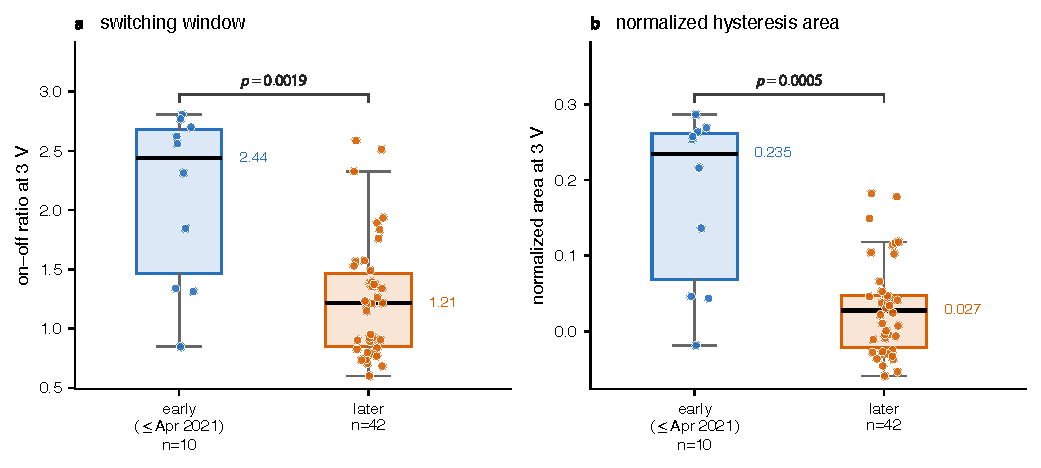
\includegraphics[width=\linewidth]{../figures/chapter3/bridge_window_collapse.pdf}
  \caption[Switching-window collapse at \texorpdfstring{$\sim$}{~}3\,V]{Switching-window collapse across the campaign on the standard \SY{}/\Hybrane{}/\LiTf{}/Ag corpus, read at the $\sim$\SI{3}{\volt} stratum where the window is expressed, one value per device. (a)~On--off ratio and (b)~normalized hysteresis area, both for devices fabricated before the NM\_v026 inflection ($\leq$Apr 2021) versus later. Boxes are quartiles; points are individual devices; the annotated $p$ is a two-sided Mann--Whitney test. The window collapses by roughly a factor of two in on--off ratio and an order of magnitude in area. Reproduced by \texttt{scripts/bridge\_figures.py} (F1).}
  \label{fig:bridge_window}
\end{figure}

\begin{table}[htbp]
  \centering
  \caption[Quantitative degradation signal]{The degradation as a multi-feature signal on the standard corpus, per device. \emph{Window collapse} is read at $\sim$\SI{3}{\volt} as an early-vs-later step at the NM\_v026 inflection (Mann--Whitney). \emph{Ohmic drift} is read at matched $\sim$\SI{1.2}{\volt} as a per-device Spearman correlation with fabrication date, reported with all dates and with the recovery tail ($\geq$2022-03) dropped; the correlation \emph{strengthens} when the reverted batches are removed, as expected if they are partial recoveries. Health flags are shown for completeness and are discussed in the text.}
  \label{tab:bridge_degradation}
  \footnotesize
  \setlength{\tabcolsep}{6pt}
  \renewcommand{\arraystretch}{1.2}
  \resizebox{\linewidth}{!}{%
  \begin{tabular}{l l l l}
    \toprule
    \multicolumn{4}{l}{\textbf{Window collapse @ $\sim$\SI{3}{\volt}} (early $\leq$Apr 2021, $n=10$ vs later, $n=42$)} \\
    \midrule
    Feature & early & later & Mann--Whitney \\
    \midrule
    on--off ratio & \num{2.44} & \num{1.21} & $p=0.0019$ \\
    normalized area & \num{0.235} & \num{0.027} & $p=0.0005$ \\
    \% change in max-V current & $+\SI{17.9}{\percent}$ & $-\SI{2.1}{\percent}$ & $p=0.013$ \\
    \midrule
    \multicolumn{4}{l}{\textbf{Ohmic drift @ matched $\sim$\SI{1.2}{\volt}} (per-device Spearman vs date, $n=64$)} \\
    \midrule
    Feature & all dates & drop recovery tail & \\
    \midrule
    current at max V & $\rho=+0.45$ ($p=0.0002$) & $\rho=+0.55$ ($p<10^{-4}$) & \\
    hysteresis area (V$\cdot\mu$A) & $\rho=+0.57$ ($p<10^{-4}$) & $\rho=+0.69$ ($p<10^{-4}$) & \\
    current difference at on--off & $\rho=+0.51$ ($p<10^{-4}$) & $\rho=+0.63$ ($p<10^{-4}$) & \\
    \midrule
    \multicolumn{4}{l}{\textbf{Health flags} (per-device, $\sim$\SI{1.2}{\volt}, $n=64$)} \\
    \midrule
    \multicolumn{4}{l}{\texttt{is\_broken} \emph{decreases} ($\rho=-0.40$, $p=0.001$) --- a handling metric, \emph{not} degradation;} \\
    \multicolumn{4}{l}{\texttt{is\_saturated} (fails to potentiate) \emph{rises} ($\rho=+0.27$, $p=0.03$).} \\
    \bottomrule
  \end{tabular}%
  }
\end{table}

\paragraph{Mechanism: ohmic drift at matched \boldmath$\sim$\SI{1.2}{\volt}.} The complementary signal lives in the conductivity, read in the tightly matched $\sim$\SI{1.2}{\volt} band so that the sweep-amplitude confound is held fixed. There, the absolute current rises with fabrication date: per device, the current at maximum voltage correlates with date at $\rho=+0.45$ ($p=0.0002$), the raw hysteresis area at $\rho=+0.57$, and the current difference at the on--off point at $\rho=+0.51$ (all $n=64$; \cref{fig:bridge_mechanism}a, \cref{tab:bridge_degradation}). Crucially, these correlations \emph{strengthen} when the deliberately-reverted recovery batches ($\geq$2022-03) are dropped --- to $\rho=+0.55$, $+0.69$, and $+0.63$ respectively --- which is exactly what one expects if those late batches are partial recoveries pulling against the underlying trend. Because the amplitude is held within a narrow band, this is a drift of the material toward more ohmic conduction, not an artefact of the sweep range. The window collapse (relative hysteresis $\to 0$) and the ohmic drift (absolute current $\uparrow$) are two faces of the same degradation. \emph{The magnitudes are deliberately reported as correlations and medians, not as a single multiplicative ``conductivity rise'', because the absolute current depends on the very sweep amplitude being controlled for.}

\begin{figure}[t]
  \centering
  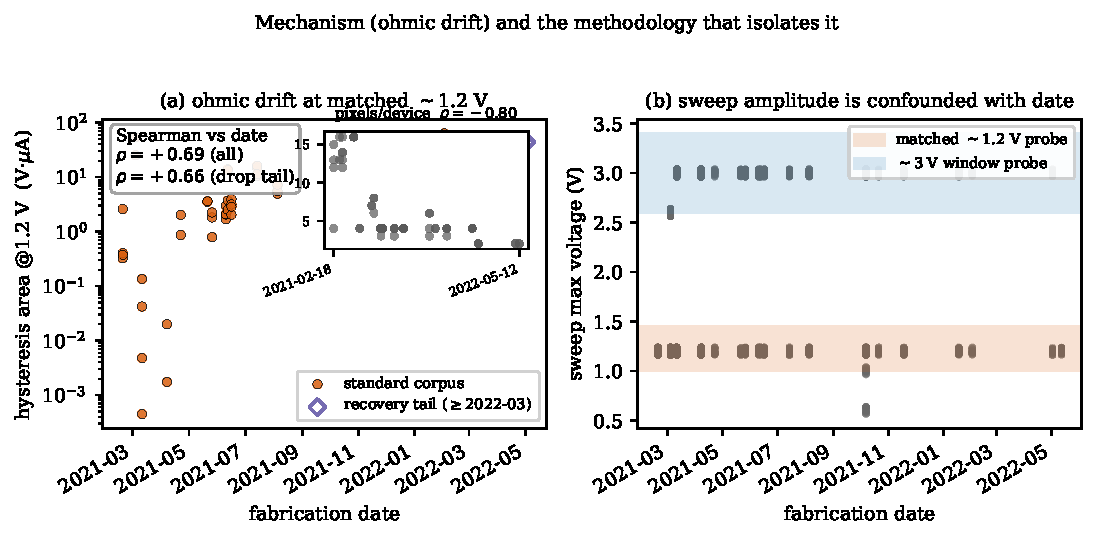
\includegraphics[width=\linewidth]{../figures/chapter3/bridge_mechanism.pdf}
  \caption[Ohmic drift and the methodology that isolates it]{Mechanism and methodology. (a)~Per-device hysteresis area read at the matched $\sim$\SI{1.2}{\volt} band rises with fabrication date (log axis; Spearman $\rho=+0.57$ over all dates, strengthening to $+0.69$ when the recovery-tail batches, open diamonds, $\geq$2022-03, are dropped). \emph{Inset:} the number of pixels measured per device falls over the campaign ($\rho=-0.80$), which is why every statistic is computed per device rather than per pixel. (b)~Sweep amplitude is itself confounded with date: the matched $\sim$\SI{1.2}{\volt} conductivity probe and the $\sim$\SI{3}{\volt} window probe (shaded) are the two strata used throughout, never pooled. Reproduced by \texttt{scripts/bridge\_figures.py} (F2).}
  \label{fig:bridge_mechanism}
\end{figure}

\paragraph{What the health flags do and do not say.} A naive degradation metric would be the fraction of broken devices; it points the wrong way. The curve-level \texttt{is\_broken} flag --- erratic or open-circuit behaviour, a contact and handling failure --- in fact \emph{decreases} over the campaign ($\rho=-0.40$, $p=0.001$), tracking the handling and contacting problems the team progressively fixed (the notes are full of them). It is therefore \emph{not} a degradation metric. The flag that does track the failure is \texttt{is\_saturated} --- a curve whose maximum current fails to exceed the previous one, i.e.\ a device that no longer potentiates --- which rises modestly with date ($\rho=+0.27$, $p=0.03$). The two flags mean different things and are reported separately so that the improvement in handling is not mistaken for the worsening of the device physics.

\subsection{A Candidate Chemistry: Moisture-Driven Hydrolytic Aging of the \Hybrane{} Stock}\label{subsec:bridge_hypothesis}

The rest of this thesis is mechanistic, so a black-box ``the stock went bad'' would be a gap a jury will rightly probe. A definitive answer, however, is \emph{not} supportable from the available record: no electrochemical impedance spectra were ever recorded on any \Hybrane{} device, no gel-permeation chromatography, nuclear-magnetic-resonance or Karl-Fischer analysis was run on the reagent stock, and the aged stock no longer exists in its degraded state. What follows is therefore presented strictly as a hypothesis together with the experiments that would confirm it.

\paragraph{The hypothesis.} \Hybrane{} is a hyperbranched polyester-amide~\cite{Froehling2004,VoitLederer2009}: ester- and amide-rich, and strongly hygroscopic. The leading hypothesis is that, over roughly a year in the bottle, the stock takes up atmospheric water and slowly hydrolyses (chain scission), and that this process could account for the measured electrical signatures without requiring a separate finished-device ageing mechanism.
\begin{itemize}
  \item \textbf{Ohmic drift} (current $\uparrow$ at matched \SI{1.2}{\volt}): absorbed water together with polar scission products raises the baseline ionic and leakage conductivity and plasticises the matrix.
  \item \textbf{Window collapse} (on--off $\to\sim$\num{1.2}, area $\to\sim$\num{0.03}, $\%\Delta I\to-\SI{2}{\percent}$): memristance needs a matrix stiff enough to \emph{hold} a field-displaced ionic profile (the metastable-polarisation picture of \cref{ch:poc}). A plasticised, lower-molecular-weight, water-laden host relaxes and leaks, so the loop closes and successive sweeps stop building up conductance.
  \item \emph{(secondary)} acidic hydrolysis products could partially dope the PPV-type \SY{}, adding a fixed, irreversible conductance --- a second route to the ``high-conductivity, undesirable'' state recorded in the notes.
\end{itemize}

\paragraph{Internal support.} Three lines of evidence already in hand are consistent with the hypothesis, though none closes it. \emph{First}, an annealing-recovery test (\cref{fig:bridge_annealing}): among late, degraded-era devices, aggressive annealing ($\geq$\SI{150}{\celsius}) restores the $\sim$\SI{3}{\volt} window to a median on--off of \num{1.95} ($n=6$) against \num{1.22} for the standard-\SI{75}{\celsius} late devices ($n=44$; Mann--Whitney $p=0.024$, one-sided), back to the early-standard reference level (\num{1.74}). Driving off absorbed water and re-densifying the film is the natural reading; a handling-only or inert-stock story does not predict a thermal recovery. \emph{This test is suggestive, not decisive:} $n=6$ elevated-temperature devices, with co-varying process tweaks, and two of them had measurement-pin issues. \emph{Second}, the full electrical fingerprint --- ohmic drift plus window and potentiation collapse --- is consistent with a water-plasticised, ion-leaky film. \emph{Third}, the material class is, by its very ester and amide linkages, intrinsically susceptible to hydrolytic chain scission, while its polar, hyperbranched architecture is hygroscopic by construction~\cite{Froehling2004,VoitLederer2009}.

\begin{figure}[t]
  \centering
  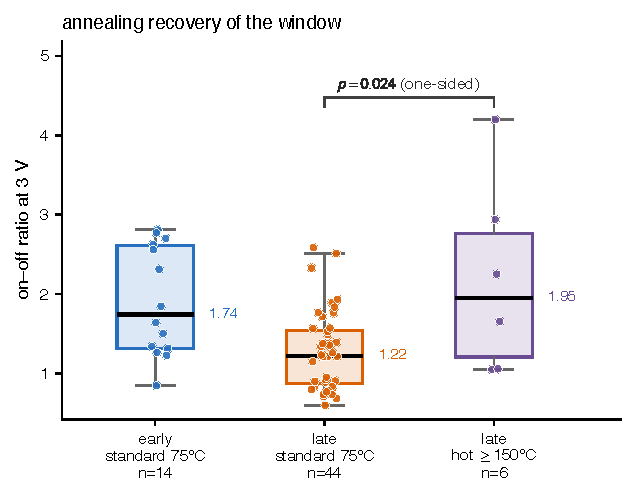
\includegraphics[width=0.62\linewidth]{../figures/chapter3/bridge_annealing_recovery.pdf}
  \caption[Annealing recovery of the switching window]{Annealing-recovery test of the hydrolysis hypothesis (\Hybrane{}/Ag, on--off ratio at $\sim$\SI{3}{\volt}, per device). Among late, degraded-era devices, an aggressive $\geq$\SI{150}{\celsius} anneal restores the window (median \num{1.22}$\to$\num{1.95}) toward the early-standard reference (\num{1.74}); one-sided Mann--Whitney $p=0.024$. Suggestive only ($n=6$ hot devices, co-varying tweaks, two with pin issues). Reproduced by \texttt{scripts/bridge\_figures.py} (F4).}
  \label{fig:bridge_annealing}
\end{figure}

\paragraph{Confirming experiments (future work).} The hypothesis would be tested directly by Fourier-transform infrared spectroscopy (loss of the ester C=O band, growth of --OH) and gel-permeation chromatography (a molecular-weight drop) on \emph{retained aged versus fresh} stock; by Karl-Fischer titration or thermogravimetry for water content; and by impedance spectroscopy to show that the ionic resistance fell. None were run on the \Hybrane{} corpus, so the hypothesis stays open --- and may never fully close, because it concerns a consumable that no longer exists in its aged state.

\FloatBarrier  % flush Table 3.2 (and §3.3 figures) before leaving the section
%% ------------------------------------------------------------
\section{The Resolution: Why PEO}\label{sec:bridge_resolution}
%% ------------------------------------------------------------

The crisis was resolved not by recovering the \Hybrane{} line but by changing the ion-transport host. Replacing the hyperbranched \Hybrane{} with linear poly(ethylene oxide) (\PEO{}) --- the host that carries the comparative study of \cref{ch:comparative} --- delivered two distinct and independently defensible wins. PEO particles are already noted entering the laboratory atmosphere by 2021-12 (NM\_v083), dating the host transition to the height of the investigation.

\paragraph{Win 1 --- a wider, stronger window.} At a matched $\sim$\SI{3}{\volt} sweep, comparing valid (non-broken, non-saturated) devices per device, the \PEO{} host opens a markedly larger switching window than the contemporaneous \Hybrane{} devices: median normalized area \num{0.26} (\Hybrane{}) $\to$ \num{0.42} (\PEO{}), Mann--Whitney $p=0.018$; median on--off ratio \num{2.45} $\to$ \num{4.91} (\cref{fig:bridge_resolution}a,b).

\paragraph{Win 2 --- temporal reproducibility, the actual solution.} This is the crisis solved. Across its full life, the \PEO{}/Ag platform \emph{sustained} a usable switching window over roughly two and a half years (2022--2024, $n=46$ devices): the per-device on--off ratio at $\sim$\SI{3}{\volt} held at a median of \num{2.61}, with yearly medians of \num{3.3}/\num{2.6}/\num{1.9} and no significant downward trend over time. The \Hybrane{} platform, by contrast, sat at a median on--off of \num{1.35} after its stock-driven collapse (\cref{fig:bridge_resolution}c). PEO simply did not exhibit the supply-degradation failure mode --- that absence, sustained over years, is the reproducibility win.

\paragraph{What ``reproducible'' means here.} The claim is precise: it is \emph{temporal / batch} reproducibility --- no stock-driven collapse over years --- and not a claim of superior within-batch, device-to-device uniformity. At matched $\sim$\SI{3}{\volt} the device-to-device coefficients of variation are only modestly different (PEO $\approx$\num{0.38} vs \Hybrane{} $\approx$\num{0.47}), and the chapter does not lean on that gap. The case for \PEO{} rests on the two wins above: a larger window and, above all, the disappearance of the supply-degradation failure over the multi-year span. The attribution of the original failure to the \Hybrane{} host stock (with \SY{} eliminated; \cref{sec:bridge_elimination}) is consistent with this resolution: changing the suspected reagent removed the failure.

\begin{figure}[t]
  \centering
  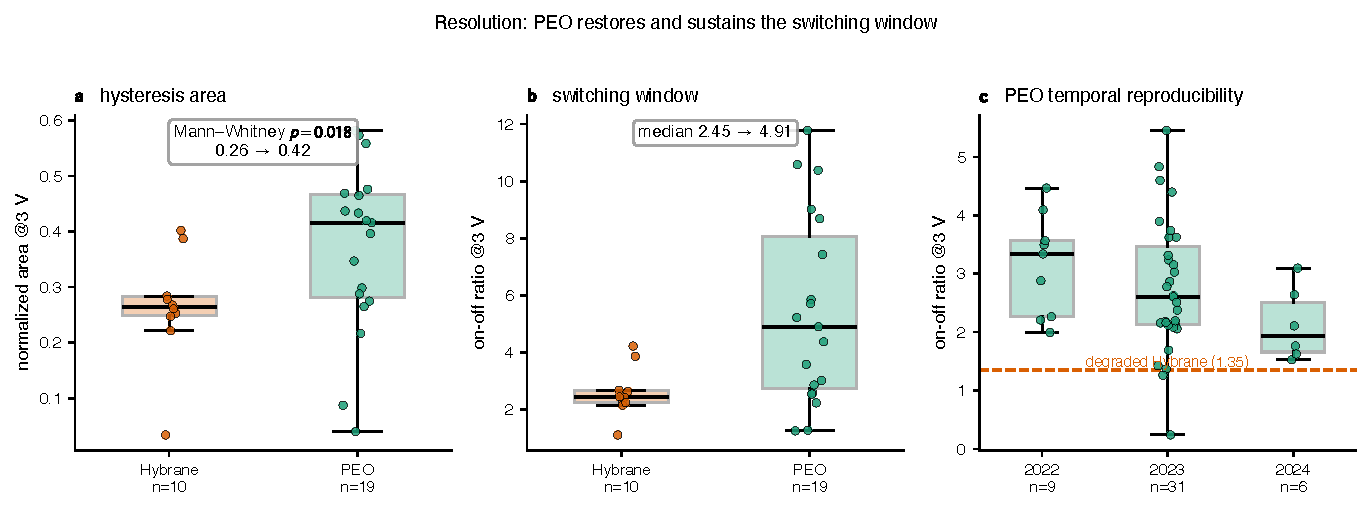
\includegraphics[width=\linewidth]{../figures/chapter3/bridge_resolution.pdf}
  \caption[PEO restores and sustains the switching window]{Resolution of the reproducibility crisis by switching to a \PEO{} host (silver electrode, $\sim$\SI{3}{\volt}, per device). (a)~Normalized hysteresis area and (b)~on--off ratio are larger for \PEO{} than for contemporaneous \Hybrane{} valid devices ($p=0.018$ for area). (c)~PEO temporal reproducibility: the per-device on--off ratio holds at a usable level (median $\approx$\num{2.6}) across 2022--2024 with no collapse, well above the degraded-\Hybrane{} level (dashed line, \num{1.35}). Reproduced by \texttt{scripts/bridge\_figures.py} (F3).}
  \label{fig:bridge_resolution}
\end{figure}

%% ------------------------------------------------------------
\section{Methodological Legacy}\label{sec:bridge_legacy}
%% ------------------------------------------------------------

The diagnosis of the previous sections required instrumentation that did not exist at the start of the campaign. Building it --- provenance capture, a normalized characterization procedure, an automated feature pipeline, and trend-discovery tooling --- is itself a contribution, and, decisively, it is the same instrumentation that produces every quantitative result in the comparative and temporal-computing chapters that follow. The crisis, in other words, paid a lasting dividend. Five durable outputs came out of it.

\begin{itemize}
  \item \textbf{A fabrication-provenance standard.} The per-device library schema (storage atmosphere, illumination, transport, reagent and solvent lots, operator, evaporation profile, and free-text fabrication and characterisation notes) exists \emph{because} the crisis forced the pinning of every variable. It made the elimination of \cref{sec:bridge_elimination} possible and is now the permanent record for every device in the archive.
  \item \textbf{A normalized electrical-characterization procedure.} A hard lesson of \cref{sec:bridge_degradation} is that the protocol sets the response: sweep amplitude alone co-determines the apparent conductivity and whether a window is even expressed. The campaign converged on fixed, documented drive and read protocols so that devices and batches are finally comparable --- the precondition for the comparative chapter.
  \item \textbf{An automated feature pipeline.} The raw instrument traces are reduced to per-device, per-pixel, and per-curve feature tables by a dedicated pipeline; every feature used in this chapter's panel, and in \cref{ch:comparative} and the temporal-computing chapter, is computed there.
  \item \textbf{Trend-discovery and curation tooling.} An interactive feature explorer (with which the present trends were originally found, and whose slicing the four controls of \cref{sec:bridge_degradation} reproduce) and a curation tool that produces the screened device set turn the archive into discoverable trendlines.
  \item \textbf{Figure generation.} A thesis-figure pipeline renders the quantitative figures from the same feature tables, so that every plotted number is traceable to the archive.
\end{itemize}

The framing is forward-looking rather than biographical: the \Hybrane{} failure is, in the end, what made the rest of the thesis measurable. The same apparatus is what the comparative study of \cref{ch:comparative} and the data-driven temporal-computing study build upon.

%% ------------------------------------------------------------
\section{Reconciliation and Bridge}\label{sec:bridge_reconciliation}
%% ------------------------------------------------------------

This chapter must be squared with \cref{ch:poc}, which attributed enhanced shelf stability to the \Hybrane{} matrix. The resolution is a partition, not a retraction, and it turns on the two-metric distinction of \cref{sec:bridge_problem}.
\begin{itemize}
  \item The \emph{published proof-of-concept device} was genuinely stable on the validated $\sim$two-week ambient shelf scale~\cite{PradoSocorro2022}; that claim stands. Indeed, \Hybrane{} \emph{devices} hold their characteristics over weeks to months --- a separate, deliberately long multi-day stability study confirms it, and is reported with the proof-of-concept device --- which is precisely why the failure here is identified as a degradation of the \emph{supply}, not of finished devices.
  \item The \emph{batch-scale reproducibility of the \Hybrane{} platform over the fabrication campaign} is a different metric, and it is the one that collapsed over the following year, in the manner quantified in \cref{sec:bridge_degradation}.
\end{itemize}
The two statements are about different axes (one device over two weeks; the fabrication line over a year) and are both true. The Chapter~\ref*{ch:poc} stability result is therefore preserved intact, and this chapter adds the campaign-scale reproducibility axis that the proof-of-concept study did not probe.

With the reproducibility crisis diagnosed and resolved by the move to a \PEO{} host, the platform is finally in a state where the volatile dynamics can be varied deliberately and compared across many nominally identical devices. That is the task of \cref{ch:comparative}, which treats the \SY{}/\PEO{}/\LiTf{} system on the silver electrode as a replicated composition grid --- using the very provenance standard, normalized protocols, and feature pipeline that this chapter's crisis brought into being --- and asks how the fading-memory dynamics can be engineered through composition and chemistry.

%% ---- Standalone close (skipped when \include'd from thesis.tex) ----
%% A unified bibliography is printed from thesis.tex in the thesis build,
%% so the per-chapter \printbibliography runs only in standalone mode.
\ifdefined\thesismode
  \let\thesisstandaloneclose\relax
\else
  \printbibliography[heading=bibintoc, title={References}]
  \def\thesisstandaloneclose{\end{document}}
\fi
\thesisstandaloneclose
